a. Modify the RBF interpolantion to include a polynomial correction. In 2D, this amounts to searching
the interpolant in the form

$$F(\bf{x}) = \sum_{j=1}^Nc_j\phi(||\bf{x}-\bf{x}_j||) + p(\bf{x})$$

where $p(x) = p(x, y) = \gamma_1 + \gamma_2x + \gamma_3y$. [See Fornberg (2016) Part 1 for details]\\

b. Solve the analogous problem in 3D, stating that given a 3D point cloud, find an implicit surface
that approximates these N points using RBF interpolants.\\

c. Revisit Exercise 1 by using the Machine Learning approach of the RBF Networks, to obtain a RBF best
fit approximation\\\\

\begin{solution}\renewcommand{\qedsymbol}{}\ \\

    a. For this problem, we will use the matrix setup in Fornberg. That is, we will calculate $A$ as we
    did in problem 1, then we will concatinate it with our $Xbig$ matrix, a ones vector, the transpose
    of these, as well as a $3\times3$ zero matrix in the lower left hand corner. Doing this along with
    adding three zeros to the end of our RHS vector allows us to solve the new system with a
    polynomial correction term. As such, we get that $\gamma_1=0.4085, \gamma_2=0.0051$, and
    $\gamma_3=-0.0009$ when using a perturbed elipse as our starting data.\\

    b. For part b, we will look at a torus with some noise. Here, we find the point cloud to be:

    \begin{center}
        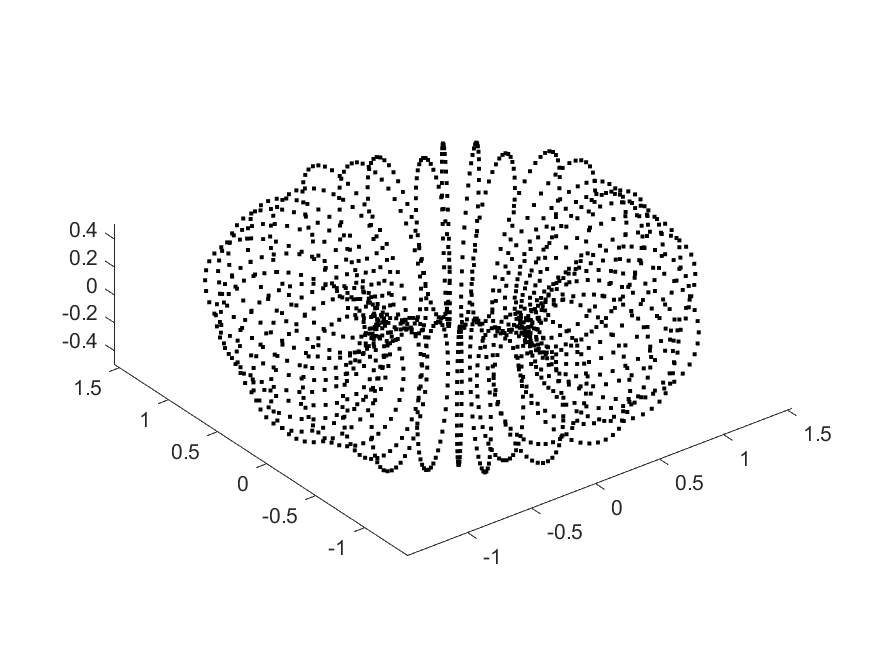
\includegraphics[scale=0.5]{problem2bcloud.PNG}
    \end{center}

    So, we then compute the normal vector at each point to get:
    
    \begin{center}
        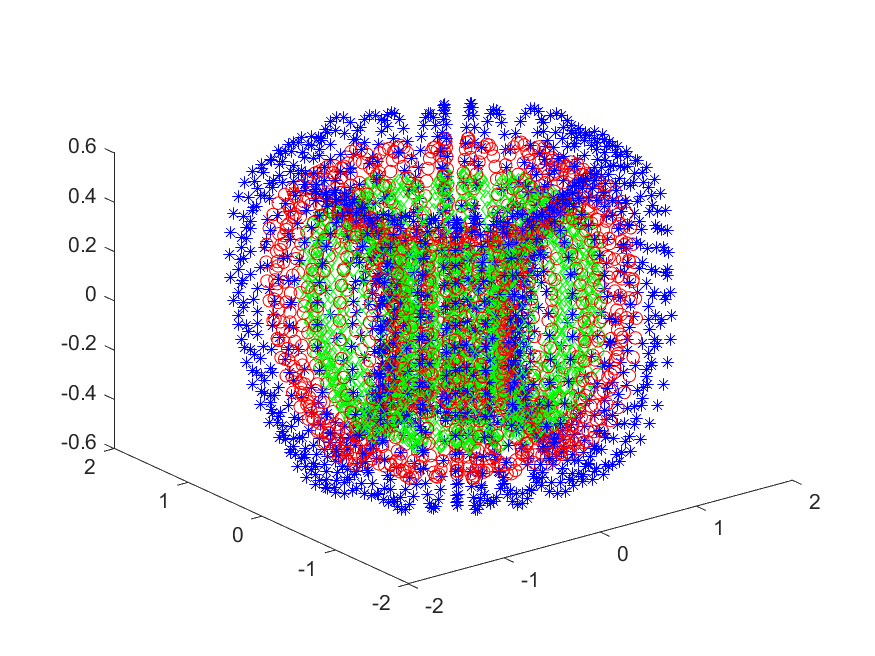
\includegraphics[scale=0.7]{problem2bnorm.PNG}
    \end{center}

    After that, we compute the interpolant as shwon in the code below. We then get the resulting level
    surface:

    \begin{center}
        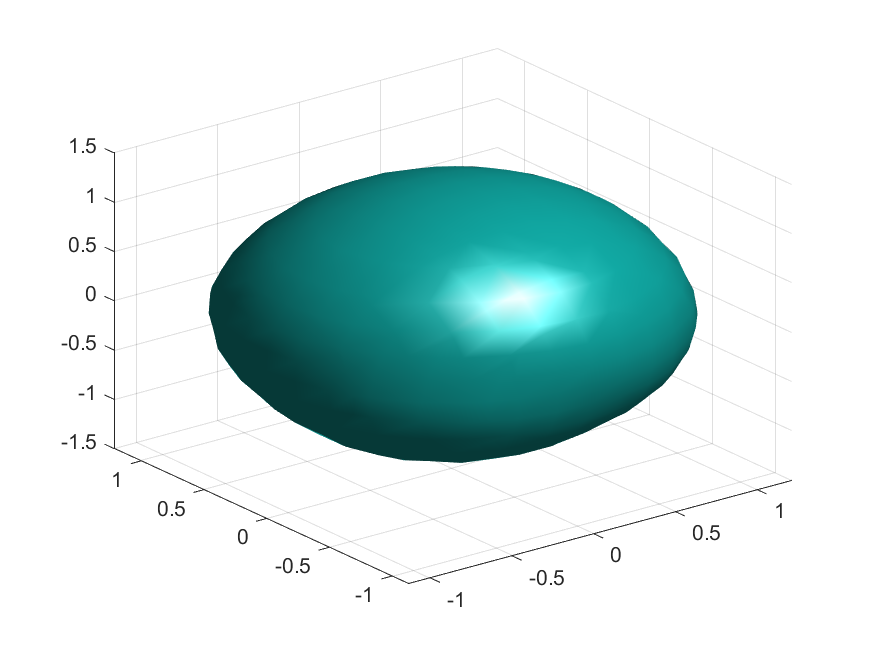
\includegraphics[scale=0.5]{problem2blvl0.PNG}
    \end{center}

    Clearly, this is not the correct level surface. This is likely due to the behavior on the inner
    radius of the torus with respect to the normal vectors. However, it still does have a sort of
    oblong shape to it, almost creating a filled in torus or an ellipsoid.\\

    c. TBD

\end{solution}

\newpage
\lstinputlisting{problem2a.m}
\newpage
\lstinputlisting{problem2b.m}